\section{Новая физика}

Несмотря на впечатляющий успех в описании экспериментов, Стандартная модель не может считаться окончательной теорией элементарных частиц. У нее есть свои трудности. Физики уверены, что она должна быть частью некоторой более глубокой теории строения микромира, той частью, которая видна в экспериментах на коллайдерах при энергиях ниже примерно 1 ТэВ. Главная задача Большого адронного коллайдера — получить хотя бы первые намеки на то, что это за более глубокая теория.

Теоретики разработали большое число кандидатов на такую теорию. Все они, естественно, включают какие-то элементы, которые отсутствуют в Стандартной модели. Часто такие теории коллективно называют «Новая физика» или «За пределами Стандартной модели». На этой странице перечислены некоторые из активно изучаемых вариантов Новой физики~\cite{2part-1}.

Суперсимметрия — это гипотетическая симметрия между фермионами и бозонами. Теории, использующие эту идею, оказываются удивительно мощными, и потому именно с суперсимметрией многие связывают надежды на открытие физики за пределами Стандартной модели. Однако до сих пор не было получено ни одного убедительного доказательства в пользу того, что суперсимметрия реализуется в нашем мире. Ее поиск является одной из главных задач Большого адронного коллайдера.
\begin{figure}
	\centering
	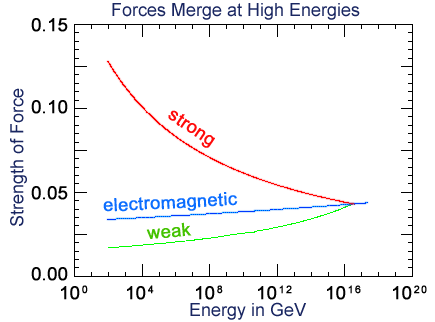
\includegraphics[width=\textwidth]{figures/hep-sm}
	\caption{Константы связи трех взаимодействий частиц}
	\label{fig:fig01}
\end{figure}
Константы связи трех взаимодействий частиц в микромире сходятся к одному значению, если имеющиеся сейчас данные экстраполировать в область очень высоких энергий. Это совпадение считается неслучайным и воспринимается физиками как намек на то, что все три взаимодействия при больших энергиях объединяются в одно.

В XIX веке физики обнаружили, что электричество и магнетизм — это две стороны одной медали, электромагнитного взаимодействия. Век спустя, при создании Стандартной модели, электромагнетизм и слабые ядерные силы были объединены в рамках единого электрослабого взаимодействия. (Точнее говоря, внутри электрослабого взаимодействия имеются по-прежнему две разные силы, а электромагнитное и слабое взаимодействия возникают как комбинации этих сил.) Каждое такое объединение упрощало теорию, уменьшало количество введенных в нее «сущностей», переводило наше понимание микромира на новый уровень.

Сейчас физики имеют сразу несколько причин подозревать, что при очень высоких энергиях происходит объединение электрослабого и сильного взаимодействий (рисунок 2.1). Модели, использующие эту идею (так называемые Теории великого объединения) разрабатываются уже давно. В идеале хотелось бы, чтобы такая теория естественным образом объясняла, почему фундаментальных взаимодействий именно столько и именно с такими свойствами, а также имела четкие предсказания, доступные проверке в современных экспериментах.

При энергиях элементарных частиц, доступных на ускорителях, гравитация по-прежнему остается исключительно слабой, так что заметить ее проявления не удается. Однако ее сила растет с ростом энергии, и при энергиях столкновения порядка планковской она станет столь же важной, как и другие взаимодействия. В этом случае в полный рост встает исключительно сложный вопрос о том, как включить гравитацию в квантовое описание микромира. Поскольку гравитация в современной физике считается проявлением кривизны пространства-времени, успешная теория с сильной гравитацией должна описывать в рамках единого формализма не только все взаимодействия и всё вещество, но и структуру пространства-времени.

Одним из наиболее привлекательных путей решения этого вопроса является теория суперструн и ее дальнейшее развитие в виде теории бран и М-теории. В этих теориях считается, что фундаментальными объектами, существующими в многомерной вселенной, являются не точечные частицы, а протяженные объекты — струны, мембраны и еще более многомерные образования. В этой теории были получены впечатляющие успехи при высоких энергиях, однако при попытке вывести свойства нашего низкоэнергетического мира из теории суперструн возникает обескураживающая неопределенность предсказаний.

Долгое время казалось, что проверка предсказаний теории суперструн лежит далеко за пределами возможностей человечества, поскольку речь идет об энергиях, на 15 порядков превышающих энергии современных ускорителей. Однако примерно 10 лет назад возникло новое направление развития теории, в котором гравитация становится сильной на энергиях порядка 1 ТэВ. Такая возможность возникает в том случае, если наш мир более чем трехмерный и если при этом новые дополнительные пространственные размерности достаточно протяженны: либо они бесконечны, либо свернуты в многомерные петельки размером много больше ядерного масштаба.

В этом случае на LHC следует ожидать целый ряд совершенно замечательных эффектов, отсутствующих в Стандартной модели, например, рождение гравитонов, которые будут улетать из нашего мира в дополнительные измерения, и микроскопических черных дыр, тут же испаряющихся с испусканием множества обычных частиц. Будут также наблюдаться сильные отклонения от предсказаний Стандартной модели в столкновении обычных частиц. Стоит, впрочем, подчеркнуть, что пока нет никаких экспериментальных подтверждений того, что эта красивая гипотеза имеет отношение к нашему миру.

Все три перечисленные выше направления «Новой физики» опираются на глубокие теоретические гипотезы об устройстве нашего мира (суперсимметрия, единство сил, квантово-гравитационная вселенная). Однако кроме этих направлений теоретики также рассматривают разнообразные теории «статусом пониже». В этих теориях просто отмечается, что текущие экспериментальные данные не запрещают те или иные экзотические объекты или явления, и разрабатываются их следствия. Вот несколько примеров таких моделей разной степени экзотичности.

\begin{figure}
	\centering
	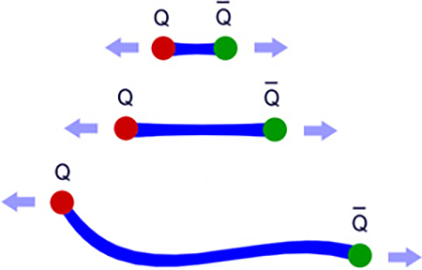
\includegraphics[width=\textwidth]{figures/quirk-antiquirk.jpg}
	\caption{Квирки}
	\label{fig:fig01}
\end{figure}

Неминимальные хиггсовские модели. Поскольку хиггсовские бозоны — единственные частицы Стандартной модели, до сих пор не открытые экспериментально, теоретики изучают самые разные варианты устройства этого сектора теории.
Новые поколения фермионов. Можно предположить, что кроме трех известных поколений кварков и лептонов существуют и другие поколения. Частицы из этих поколений должны быть очень тяжелыми, иначе бы их уже давно открыли в эксперименте.

Новые короткодействующие силы. В таких моделях предполагается, что в нашем мире есть и иные силовые взаимодействия, отличные от сильных, слабых и электромагнитных, но они настолько короткодействующие, что до сих пор никак не проявлялись в эксперименте. На Большом адронном коллайдере благодаря его рекордной энергии удается «прощупать» взаимодействия частиц на исключительно малых расстояниях (менее 10–19 метра), а значит, появляется шанс эти взаимодействия обнаружить. Они могут проявляться либо как рождение и распад частицы-переносчика новых сил (такие гипотетические частицы обозначают Z'), либо как усиленное рассеяние частиц на большие углы.

Лептокварки. В Стандартной модели и в подавляющем большинстве теорий Новой физики кварки и лептоны взаимодействуют друг с другом опосредованно, путем обмена квантами силовых полей. Однако можно представить себе возможность того, что кварки и лептоны исходно являлись фермионами одного типа и лишь потом расщепились на два разных сорта. В таком случае должны существовать новые тяжелые частицы — лептокварки, — которые распадаются прямо на кварк и лептон. Подобные частицы встречаются в теориях Великого объединения.

Квирки. Одним из очень необычных и любопытных вариантов новых сил является гипотеза квирков (quirks). Эта модель построена по типу обычного сильного взаимодействия: в ней предполагается, что существует новое силовое поле с конфайнментом и новые частицы, его чувствующие. Если частицы очень тяжелые, то между ними будут натягиваться длинные, даже макроскопические силовые струны, которые не смогут порваться (рисунок 2.2).




